\documentclass[../full_thesis/full_thesis.tex]{subfiles}

% Default image directory
\newcommand{\thisdir}{../detecting_cgw}
\graphicspath{{\thisdir/img/}}

\begin{document}

Timing variations, in the form of glitches or timing-noise, pose a serios risk
to efforts to discover continuous GWs from neutron stars due to the fact that
searches rely on \emph{matched-filtering}. In this section we will give a
general introduction to detection methods used in GW data analysis, explain why
timing variations pose a risk, and introduce some simple calculations. The
details of estimating the risk for glitches and timing noise will be covered in
Chapter~\ref{sec: glitches in cgw} and Chapter~\ref{sec: timing noise in cgw}.

\section{Introduction}
\meta{Greg: Add introduction from either paper}

\section{Introduction to the mismatch}
\meta{Greg: Add Sec IV from glitch paper}

\section{Mismatch from discreet offsets in the GW phase}

The $\mathcal{F}$-statistic considered in \citet{Brady1998} analytically
minimises over the phase. Therefore if the signal and template can both be
modelled by a single smooth Taylor expansion, but with a finite phase-offset,
the mismatch is zero: the mismatch is insensitive to any overall phase
difference between the signal and template. However, a mismatch will occur if
the overall phase between the signal and template changes during an
observation. In this section we will investigate three scenarios where this
occurs. While not all these scenarious are physically relevant to real astrophysical
systems, this introduces some concepts in a simple setting before we tackle
the more difficult real astrophysical systems.

\subsection{Two subdomains with a phase discontinuity}
\label{sec: Two segments with a phase offset}

We begin with a simple system in which the signal undergoes an instantaneous
`jump' in its GW phase halfway through the observation. We can model this
signal by a \emph{piecewise} Taylor expansion with two subdomains.
\meta{Greg: Should move definitions of things here?}. Both
subdomains are of equal duration and follow a smooth spindown except that
there is a phase discontinuity at their interface; we illustrate this setup
in Fig.~\ref{fig: PhaseJump}.
\begin{figure}[htb]
    \centering
    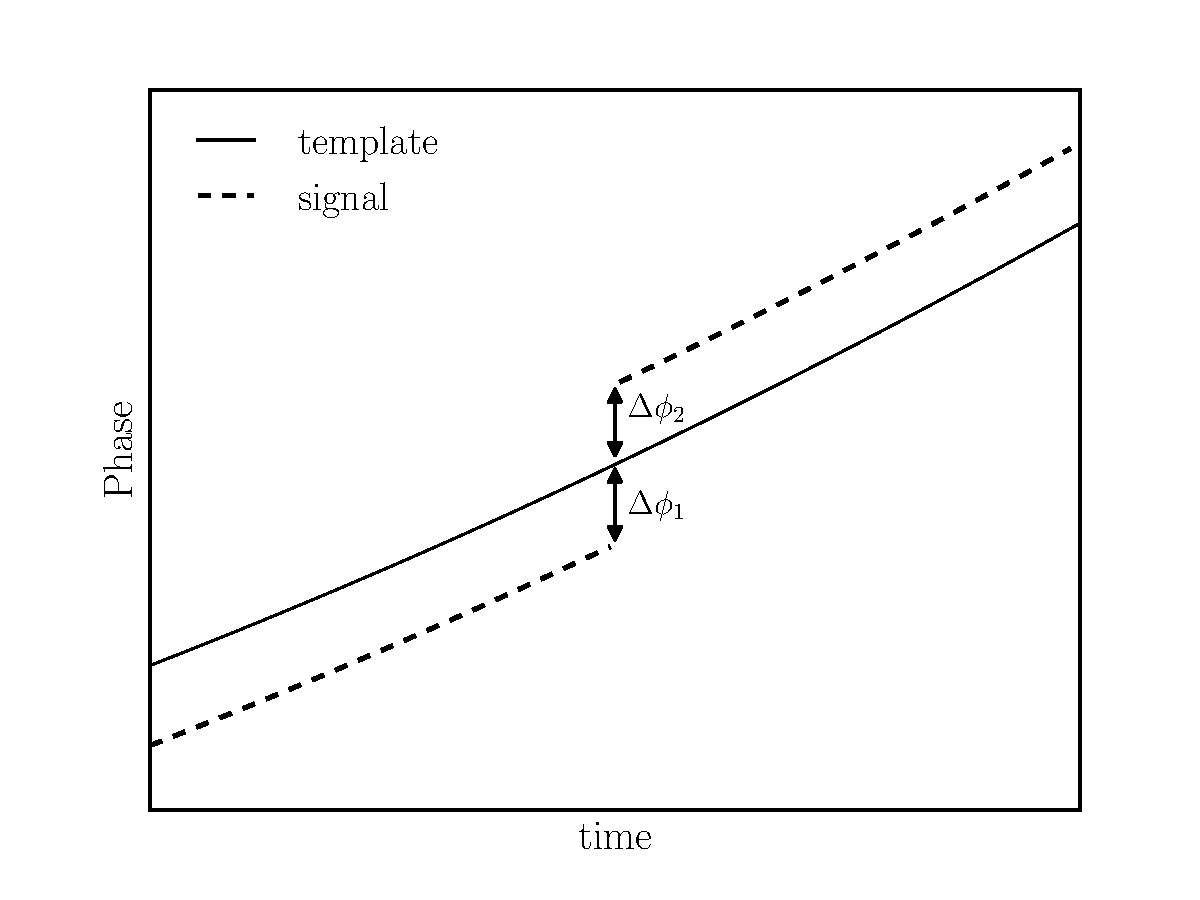
\includegraphics[width=.5\textwidth]{PhaseJump}
    \caption{Illustration of the signal and template defined in equation
        \eqref{eqn: phase offset}}
    \label{fig: PhaseJump}
\end{figure}
Parameterising by the offset with respect to the template $\bl_{0}$ for some
arbitrary template and phase jump, we write the phase deviations in the two
subdomains as
\begin{equation}
 \Delta\Phi(t) = \left\{
\begin{array}{cr}
\Delta \phi_{1}& \; 0 < t < T/2 \\
\Delta \phi_{2} & \;  T/2 < t < T
\end{array}.
\right.
\label{eqn: phase offset}
\end{equation}

To compute the matched filtering amplitude given in Eqn.~\eqref{eqn: matched
filtering amplitude}, we can factorise the integral using the additivity of
integration on intervals into two integrations
\begin{eqnarray}
X & = &\frac{1}{T } \int_{0}^{T}e^{i\Delta\Phi(t)} dt\\
 & = &\frac{1}{T }\left(\int_{0}^{T /2}e^{i\Delta\phi_{1}} dt  +
\int_{T/2}^{T} e^{i\Delta\phi_{2}}dt\right)\\
& = & \frac{1}{2}\left(e^{i\Delta\phi_{1}} + e^{i\Delta\phi_{2}}\right).
\end{eqnarray}
Because our choice in splitting up the integral exactly matches the sub-domans
defined in Eqn.~\eqref{eqn: phase offset}, and in each sub-domain $\Delta\Phi(t)$
is constant, we can compute the integrals.
The absolute square value of the matched filtering amplitude is then
\begin{eqnarray}
|X|^{2}& = &\frac{1}{4}\left(e^{i\Delta\phi_{1}} + e^{i\Delta\phi_{2}}\right) \left(e^{-i\Delta\phi_{1}} + e^{-i\Delta\phi_{2}}\right)\\
& = &\frac{1}{4} \left(2 + e^{i(\Delta\phi_{1} - \Delta \phi_{2})} +  e^{-i(\Delta\phi_{1} - \Delta_{\phi_{2}})} \right) \\
& = &\frac{1}{2}\left(1 + \cos(\Delta\phi_{1} - \Delta\phi_{2})\right).
\end{eqnarray}
Finally, the mismatch can be calculated from equation \eqref{eqn: full mismatch}.
\begin{equation}
\mu = \frac{1}{2}\left(1 - \cos(\Delta\phi_{1} - \Delta\phi_{2})\right).
\label{eqn: two segment phase mismatch}
\end{equation}

From this result we learn that it is not the phase difference with respect to
each of the Taylor expansion ($\Delta\phi_1$ or $\Delta\phi_2$) which is
important, but the total phase jump at their interface. For $\Delta \phi_{1} =
\Delta \phi_{2}$ the mismatch vanishes, this recovering the case of a single
Taylor expansion signal with an arbitary overall phase offset which always has
zero mismatch. This result can be used to calculate the mismatch due to a glitch,
if the glitch is purely in the phase; in reality we know that glitches are
discontinuities in the frequency and spin-down rate which will be considered in
Chapter~\ref{sec: glitches in cgw}.

\paragraph{Comparing with an exact numerical result}
\meta{Greg: potentially cut this} We can verify equation
\eqref{eqn: two segment phase mismatch} by comparing with the results of a
exact numerical calculation of the mismatch. This involves defining the signal
such that it describes two segments with a phase offset, then `injecting' and
recovering the signal using \texttt{LALApps} software. We do this in the
absence of noise and compute the mismatch against a perfectly matched signal.
The signal comprises two adjacent transient windows of fixed duration. We set
the phase offset in the first segment to zero and subject the second segment to
a phase jump $\Delta \phi$, therefore
\begin{align}
    \Delta \phi_{1} &= 0 &  \textrm{ and } && \Delta \phi_{2} =& \Delta\phi.
\end{align}
Varying $\Delta\phi$ we plot the exact numerical result along with the
prediction of equation~\eqref{eqn: two segment phase mismatch} in
Fig.~\ref{fig: two plot}
\begin{figure}
\centering
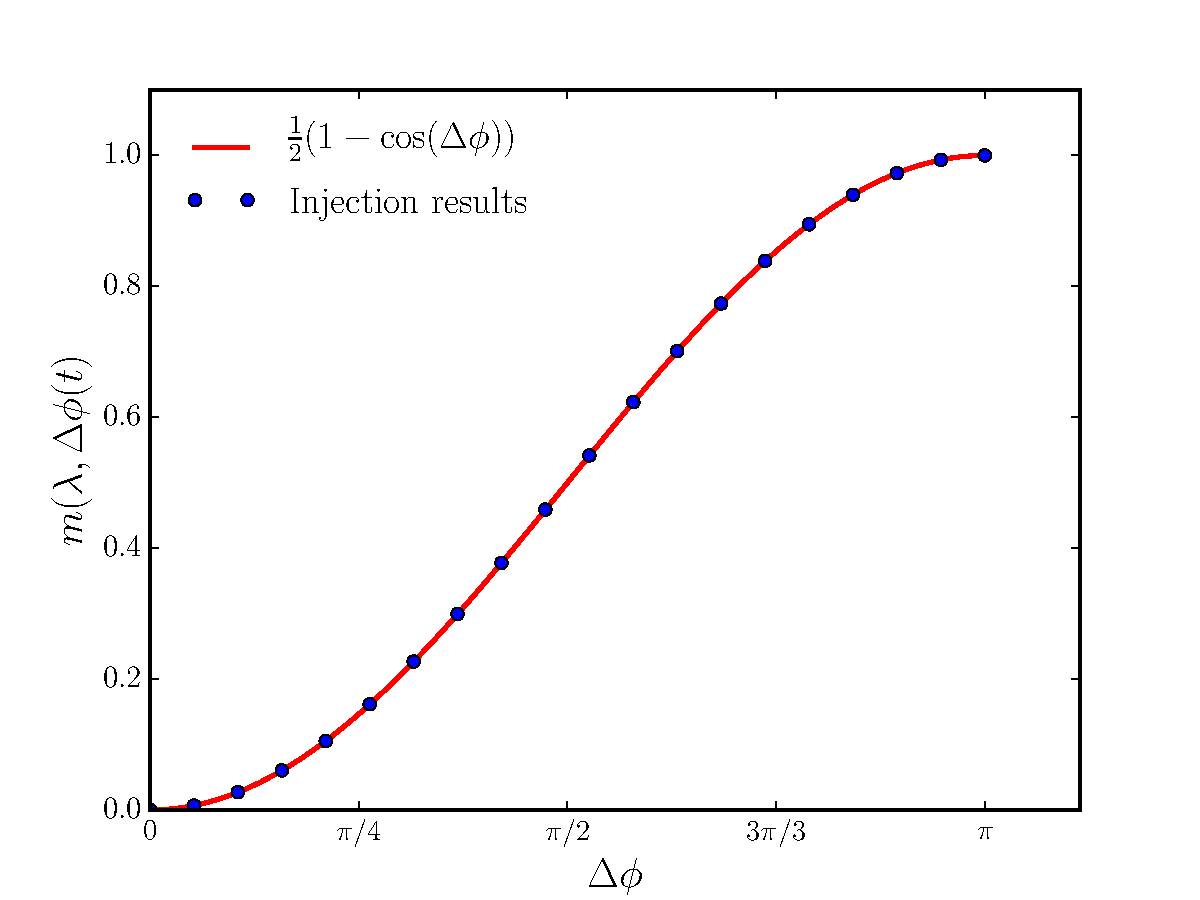
\includegraphics[width=0.65\textwidth]{Exact_analytic_phase_two_segments}
\caption{Plot of the theoretical prediction of equation~\eqref{eqn: two segment
phase mismatch} given a time dependent phase offset as in equation\eqref{eqn:
phase offset}. This is compared  with a signal injection and recovery
using \texttt{LALapps} software.}
\label{fig: two plot}
\end{figure}

\subsection{N subdomains with phase discontinuity's}
We can further generalise Eqn.~\eqref{eqn: two segment phase mismatch} by
letting the signal be comprised of $N$ equal duration subdomains with a phase discontinuity
$\Delta\phi_i$ for the $i^{th}$ subdomain.
Then, the matched filtering amplitude can be written
\begin{eqnarray}
X & = & \frac{1}{T}\left(\int_{0}^{t_{1}}e^{i\Delta\phi_{1}} dt +
\int_{t_{1}}^{t_{2}}e^{i\Delta\phi_{2}} dt + \dots +
\int_{t_{N-1}}^{t_{N}}e^{i\Delta\phi_{N}} dt \right) \\
& = &  \frac{1}{T}\left(\frac{T}{N}e^{i\Delta\phi_{1}} +
\frac{T}{N}e^{i\Delta\phi_{2}} + \dots + \frac{T}{N}e^{i\Delta\phi_{n}} \right)\\
& = & \frac{1}{N} \sum_{i=1}^{N}e^{i\Delta \phi_{i}}.
\end{eqnarray}
Squaring the matched filtering amplitude and simplifying
\begin{eqnarray}
|X|^{2} & = &  \frac{1}{N^{2}} \left(\sum_{i=1}^{N}e^{i\Delta \phi_{i}}\right)\left(\sum_{j=1}^{N}e^{-i\Delta \phi_{j}}\right) \\
|X|^{2} & = &  \frac{1}{N^{2}} \sum_{i=1}^{N}e^{i\Delta \phi_{i}}\left(\sum_{j=1}^{N}e^{-i\Delta \phi_{j}}\right) \\
& = & \frac{1}{N^{2}} \sum_{i=1}^{N}e^{i\Delta \phi_{i}}\left(e^{-i\Delta \phi_{i}} +  \sum_{\substack{j=1 \\j\ne i}}^{N}e^{-i\Delta \phi_{j}}\right) \\
& = & \frac{1}{N^{2}} \left(\sum_{i=1}^{N}1 +   \sum_{i=1}^{N}\sum_{\substack{j=1 \\j\ne i}}^{N}e^{i(\Delta\phi_{i}-\Delta \phi_{j})}\right) \\
& = & \frac{1}{N^{2}} \left(N +   \sum_{i=1}^{N}\sum_{\substack{j=1 \\j\ne i}}^{N}\cos(\Delta\phi_{i} - \Delta\phi_{j}) + i\sin(\Delta\phi_{i} - \Delta\phi_{j})\right).
\end{eqnarray}
In this final summation for each pair $(i,j)$ the corresponding pair $(j, i)$
will exist in the sum. This leads to a cancellation of the imaginary part and a
doubling of the real part
\begin{equation}
|X|^{2}  = \left(\frac{1}{N} + \frac{1}{N^{2}}\sum_{i=1}^{N}\sum_{\substack{j=1 \\j\ne i}}^{N} \cos(\Delta\phi_{i} - \Delta \phi_{j})\right).
\end{equation}•
Then the mismatch is given by:
\begin{equation}
\mu = 1 - \frac{1}{N} - \frac{1}{N^{2}}\sum_{i=1}^{N}\sum_{\substack{j=1 \\j\ne i}}^{N} \cos(\Delta\phi_{i} - \Delta\phi_{j}).
\label{eqn: phase mismatch}
\end{equation}

This result could be used to estimate the mismatch due to a random walk model
of timing noise where the random walk was purely in the phase (see
Sec.~\ref{sec: TN interpretations random walk models} for example)

\subsection{Oscillating phase deviations}

Timing residuals, or equivalently the phase offsets between Taylor expansions
and the real signals, are often found to have a quasi-periodic structure
\citep{Hobbs2010}. It is reasonable to ask if, because the residuals oscillate
about the origin, the loss of detection will be cancelled out. In this section
we consider such an oscillating phase deviation and show that, over many
oscillations, the mismatch is non-zero.

We model a small sinusoidal phase offset by a trigonometric function
\begin{equation}
\Delta \Phi(t) = \varepsilon \cos(\omega t),
\end{equation}•
where $\varepsilon$ is the amplitude of variatinos and $\omega$ is the angular
frequency of the oscillations. If we assume that the variations are small
$\varepsilon \ll 1$, we can Taylor expandthe exponential phase offset in
the matched filtering amplitude
\begin{equation}
X = \frac{1}{T}\int_{T}
1 + i \epsilon \cos{\left (\omega t \right )}
- \frac{\epsilon^{2}}{2} \cos^{2}{\left (\omega t \right )}
- \frac{i \epsilon^{3}}{6} \cos^{3}{\left (\omega t \right )}
dt
+ \mathcal{O}\left(\epsilon^{4}\right).
\end{equation}
Inserting this into equation~\eqref{eqn: full mismatch} and computing the
mismatch we find
\begin{equation}
\mu = \varepsilon^{2} \left(\frac{1}{2}
+ \frac{\sin{\left (2 T \omega \right )}}{4 T \omega}
+ \frac{\sin^{2}{\left (T \omega \right )}}{T^{2} \omega^{2}} \right)
+ \mathcal{O}\left(\epsilon^{4}\right).
\label{eqn: Oscillating mismatch}
\end{equation}
In the limit $T \rightarrow \infty$ this tends to $\varepsilon^{2}/2$. Before
this, the mismatch oscillates around this value over observation times similar
to the oscillation period; this is shown in figure \ref{fig:
OscillatoryPhaseMismatch}.
\begin{figure}[ht]
\centering
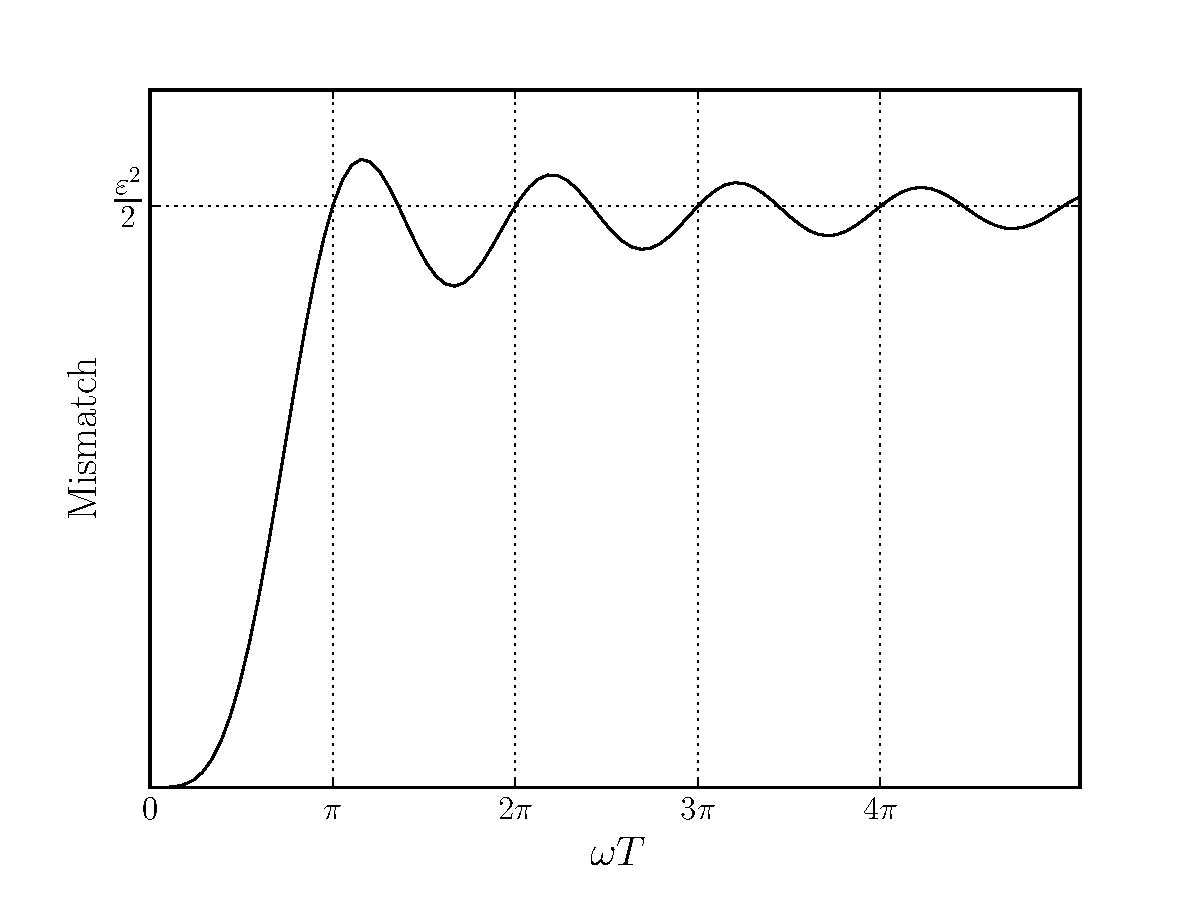
\includegraphics[width=.6\textwidth]{OscillatoryPhaseMismatch}
\caption{Plot demonstrating the behaviour of equation
         \eqref{eqn: Oscillating mismatch}, the mismatch for an oscillating
         phase offset.}
\label{fig: OscillatoryPhaseMismatch}
\end{figure}

This simple model demonstrates that if the signal and template are on average
coherent, but the phase residual between them oscillates about the mean, then
over several cycles the mismatch will approach a constant value dependent on
the maximum amplitude of the residuals.  For a quasi-periodic signal the same
overall picture will emerge with the size of the mismatch dependent on the mean
average size of oscillations in the residual.

\biblio


\end{document}
